It is possible to calculate the fastest route between point A and B If we add the parameters $v_1$, $v_2$, $\theta _1$, $\theta _2$, $a$, $b$, $c$ and $d$ which corresponds respectively to the propagation speed on the beach, the propagation speed in the water, the angle of the path on the beach with the normal, the angle of the path in the water with the normal and distances which can be seen in figure \ref{fig_snell_full}.

\begin{figure}[h!]
	\centering
	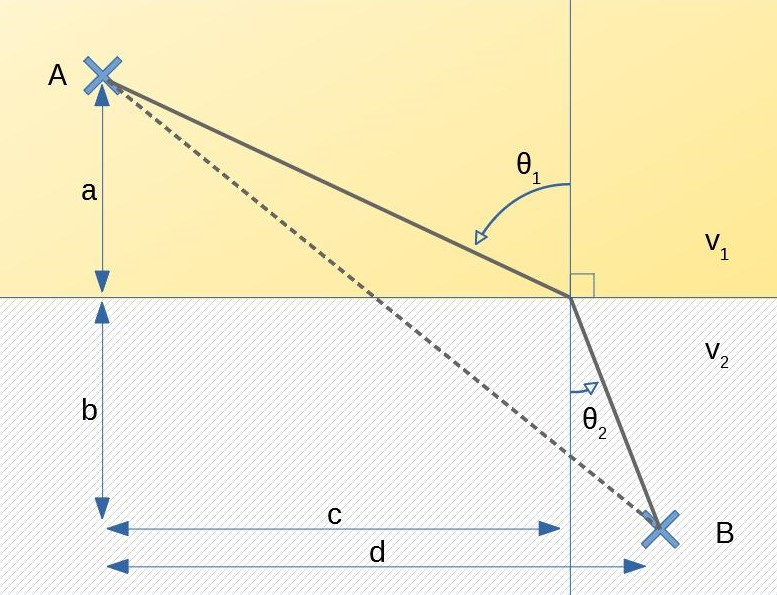
\includegraphics[width=8cm]{afbeeldingen/snell_diagram_vol.jpg}
	\caption{Diagram of beach analogy with parameters $v_1$, $v_2$, $\theta _1$, $\theta _2$, $a$, $b$, $c$ and $d$. These correspond respectively to the propagation speed on the beach, the propagation speed in the water, the angle of the path on the beach with the normal, the angle of the path in the water with the normal and distances which can be seen in the diagram.}
	\label{fig_snell_full}
\end{figure}

The time it takes to travel from point A to B, $t$, can easily be found dividing the path on the beach and the water, respectively $l_{beach}$ and $l_{water}$ by the corresponding speed:

\begin{equation*}
	t = l_{beach}/v_1 + l_{water}/v_2
\end{equation*}

Using the pythagoras theorem we find:

\begin{equation}
	t = \sqrt{a^2 + c^2}/v_1 + \sqrt{b^2 + (d-c)^2}/v_2
	\label{eq_t}
\end{equation}

If there is a fastest path, there should be an optimum value for $c$ for which $dt/dc = 0$. Therefore, applying the principle of Fermat to equation \ref{eq_t} leads to the following:

\begin{equation*}
	0 = \frac{c}{v_1 \sqrt{a^2 + c^2}} + \frac{c-d}{v_2 \sqrt{b^2 + (d-c)^2}}
\end{equation*}

We now need the following trigonometric identity for right-angled triangles:
 
\begin{equation}
	sin(\theta) = (adjacent side)/(diagonal side) 
	\label{eq_sin_identity}
\end{equation}

Filling in this identity yields:

\begin{equation*}
	0 =  sin(\theta _1)/v_1 - sin(\theta _2)/v_2
\end{equation*}

If we rewrite this and use the fact that the speed of light in a medium is given by $v = c/n$ we obtain Snell-Descartes law:

\begin{equation*}
	n_1 \; sin(\theta _1) = n_2 \; sin(\theta _2)
\end{equation*}

This equation basically tells us, that for a interface to a higher refractive index, so where the light slows down, the light bends towards the normal.